\documentclass[review,number,sort&compress]{elsarticle}
\usepackage{amsmath,amssymb}
\usepackage{graphicx}
\usepackage{booktabs}
\usepackage{multirow}
\usepackage{tabularx}
\usepackage{xcolor}
\usepackage{xeCJK}
\setCJKmainfont{Noto Serif SC}
\setCJKsansfont{Noto Sans SC}
\usepackage[colorlinks=true,linkcolor=blue,citecolor=blue,urlcolor=blue]{hyperref}
\journal{Applied Acoustics}

\newcommand{\cer}{\mathrm{CER}}
\newcommand{\wer}{\mathrm{WER}}

\begin{document}
\begin{frontmatter}

\title{Error Propagation in Cascaded Speech Translation under Acoustic Channel
Degradations: A Black-Box Case Study of Commercial Speech Intelligence APIs}

\author[addr1]{Anonymous Author}
\address[addr1]{Affiliation withheld for double-blind review}

\begin{abstract}
Cloud speech services are consumed as black boxes, yet the acoustic channels
feeding them are rarely clean. We present CascadeBench, a fully seeded
black-box benchmark that measures how twelve controlled acoustic channel
degradations propagate through the recognition and translation stages of
commercial speech APIs: five recognition systems spanning three product
classes of a single provider (specialised streaming, audio-LLM, and
omni-modal), two cascaded and two end-to-end speech translation paths, over
a symmetric 480-sentence Mandarin--English corpus with a babble severity
sweep from 20 to $-10$~dB. Recognition error rises as a knee-shaped
function of noise level: the audio-LLM systems hold a flat sub-percent
floor and tolerate 2.5 to 4~dB more noise than the specialised streaming
system before error reaches ten percent, but collapse sharply below 0~dB,
where insertion-heavy hallucination drives character error rates above 100
percent. A telephone-band specialist shows no in-band advantage and is
uniquely fragile under reverberation. Cascade translation quality falls
linearly with recognition error rate (0.44 to 0.54 BLEU points per
percentage point, sentence-level bootstrap 95\% confidence intervals within
$\pm 0.04$, intercept indistinguishable from zero) across fifteen operating
conditions. End-to-end translation is not automatically more robust: under
0~dB babble the omni-modal path loses a third of its BLEU score, more than
a well-frontended cascade, whereas a streaming end-to-end service is the
most resilient path measured. A dual-reference protocol exposes a
machine-reference scoring bias that can invert system rankings. The
complete recipe, corpus, degraded audio, and 33{,}000 logged API responses
are released for re-measurement as services evolve.
\end{abstract}

\begin{keyword}
speech recognition \sep speech translation \sep robustness benchmark \sep
acoustic channel degradations \sep cascaded systems \sep cloud APIs
\end{keyword}

\end{frontmatter}

\section{Introduction}
\label{sec:intro}

Speech has become a primary interface to cloud intelligence. Voice assistants,
meeting transcription products, live captioning services, and multilingual
communication platforms are routinely assembled from commercial automatic
speech recognition (ASR) and machine translation (MT) interfaces offered by
large cloud providers. In a typical deployment, audio captured by a far-field
microphone or transported over a communication channel is first converted to
text by an ASR service, and the resulting text is then passed to a text
translation engine whenever the application crosses a language boundary. This
cascade architecture dominates industrial practice because it allows each
stage to be selected, replaced, and billed independently, and because the best
available components at each stage are often operated by different providers.
An alternative architecture, end-to-end speech translation (E2E ST), maps
source-language audio directly to target-language text and has matured
rapidly with large foundation models.

The acoustic pathway between a speaker and these services is rarely pristine.
Speech arrives mixed with competing talkers, shaped by room reverberation,
band-limited by telephone channels, compressed by low-bitrate codecs, or
corrupted by packet loss on unstable network links. The robustness of ASR
systems to such degradations has been a central concern of the speech research
community for decades, and controlled robustness corpora have driven
substantial progress. What has changed is the identity of the systems that
now dominate deployment. Commercial speech services are increasingly built on
large language model (LLM) based ASR, on general-purpose multimodal foundation
models that accept audio alongside text, and on streaming speech translation
models, none of which can be fine-tuned, inspected, or benchmarked offline by
their consumers. A systems integrator who composes such services into a
translation pipeline has no principled way to predict how recognition errors
induced by an acoustic channel will propagate into the final translation, or
whether a cascade or an end-to-end design is the safer choice under the
conditions of a given deployment.

The evaluation gap is not academic. Deployment decisions are made
weekly by integrators who must choose among service tiers and architectural
patterns with nothing but clean-audio demo pages and marketing claims, while
the operating conditions of real audio pathways, conference rooms, vehicles,
telephone trunks, and congested wireless links, are precisely the conditions
that clean demos do not exercise. A deployment that selects a recognition
frontend on clean-audio accuracy alone can be quietly losing most of its
translation quality in the field, and a deployment that assumes end-to-end
robustness can be more fragile than the cascade it replaced. Closing this
gap requires measurement that is controlled at the acoustic layer, complete
at the pipeline layer, and reproducible at the service layer, and that is
the design brief of the benchmark presented here.

This gap motivates the present study. Academic robustness benchmarks such as
Aurora~\cite{pearce2000aurora} and the CHiME challenge
series~\cite{barker2018fifth} evaluate open recognizers on fixed noise
corpora, but they do not cover the black-box commercial systems that now carry
production traffic, they rarely extend beyond recognition to the downstream
translation stage, and they cannot be re-run on new model versions without
access to model internals. Conversely, studies that compare commercial ASR
services report error rates on fixed test sets but typically consider clean
audio and stop at the transcription boundary. The propagation of acoustic
degradation through a complete speech translation pipeline, comparing
architectural families and both cascade and end-to-end designs under
identical and fully controlled channel conditions, has to our knowledge not
been quantified for the current generation of speech APIs.

This paper presents CascadeBench, a black-box benchmark designed to answer
four questions. First, how sensitive are the main product classes of
commercial ASR, namely specialised streaming models, LLM-based recognisers,
and general-purpose multimodal models, to eight canonical acoustic channel
degradations? Second, how does recognition accuracy scale with noise
severity across the full range from mild to destructive, and where does
each class fail? Third, when
recognition errors flow into a downstream translation engine, does the
cascade amplify them, and how does the cascade compare with end-to-end speech
translation under identical conditions? Fourth, what are the latency
consequences of each choice? To answer these questions under the
constraint that only public interfaces are available, the benchmark
synthesises a stratified bilingual corpus of 480 Mandarin Chinese and English
sentences with multiple neural voices, applies a grid of eight controlled
acoustic degradations together with an eight-level noise severity sweep from
20 to $-10$~dB, and measures five recognition systems, three cascade
translation paths, and two
end-to-end speech translation paths through their public APIs, using only
free service quotas. All systems come from one provider, so the study is a
single-provider case study whose class-level findings require cross-provider
replication before attribution to architecture; this constraint is examined
in Section~\ref{sec:limitations} and revisited throughout.

The study yields findings that are relevant to both the science of robust
speech processing and the practice of assembling speech services. Recognition
services from the three classes differ sharply in where, rather than how
fast, they fail under noise: the LLM-based recognisers hold a sub-percent
error floor and cross ten percent error at noise levels 2.5 to 4~dB lower
than the specialised streaming system, with sharper collapse beyond their
knee, and below 0~dB they fail by insertion-heavy hallucination that drives
character error rates above 100 percent. The end-to-end translation paths,
often assumed to be more robust
than cascades because they avoid error propagation, do not inherit
robustness automatically: the omni-modal path loses more of its clean
quality under severe noise than a well-frontend cascade, while a streaming
end-to-end service is the most resilient path measured. Across fifteen
operating conditions, the BLEU score of every cascade measured
falls linearly with its recognition error rate, with a pass-through slope of
0.44 to 0.54 BLEU points per percentage point, sentence-level bootstrap
confidence intervals within $\pm 0.04$, and an intercept statistically
indistinguishable from zero, which gives integrators a calibrated
engineering rule for estimating translation losses from recognition
quality alone. Finally, the benchmark surfaces behavioural differences that
are invisible in clean-audio evaluations, including two distinct
empty-output mechanisms under severe noise, an explicit protocol-level
refusal and a silent empty return, and the unique fragility of a
telephone-band specialist under reverberation.

The contribution of this paper is threefold. It provides, to our knowledge,
the first systematic measurement of acoustic degradation propagation across
recognition and translation stages for commercial black-box speech APIs,
covering three product classes of one provider and both cascade and
end-to-end translation designs, which we frame as a case study pending
cross-provider replication. It introduces a fully reproducible benchmark
recipe in which the test material, the degradations, and every model response
are controlled, logged, and released, so that the measurements can be
repeated as providers update their models. And it distils the measurements
into quantitative design guidance, including noise-failure thresholds per
product class, the error pass-through regression for cascades, and a
dual-reference protocol that exposes and controls the systematic bias that
arises when automatic translation quality is scored against references
produced by models related to one of the systems under test.

The remainder of the paper is organised as follows.
Section~\ref{sec:related} reviews related work on robust ASR, cascade and
end-to-end speech translation, and the evaluation of commercial services.
Section~\ref{sec:methods} describes the benchmark design, including the
corpus, the degradation grid, the systems under test, and the evaluation
protocol. Section~\ref{sec:results} presents the results, and
Section~\ref{sec:discussion} discusses their implications for practitioners
and for future evaluation practice. Limitations are examined in
Section~\ref{sec:limitations}, and Section~\ref{sec:conclusions} concludes.

\section{Related work}
\label{sec:related}

\subsection{Robustness of speech recognition under acoustic degradation}

The sensitivity of ASR to noise and channel distortions has been studied since
the earliest statistical recognisers~\cite{lippmann1997speech}. Surveys such
as that of Virtanen et al.~\cite{li2014overview} organise this
literature around feature enhancement, model adaptation, and multi-condition
training. Controlled evaluation infrastructure has been decisive for
progress. The Aurora framework~\cite{pearce2000aurora} standardised noise
types and signal-to-noise ratios for telephone-band recognition, and the CHiME
challenge series~\cite{barker2018fifth} extended such evaluation to
far-field, reverberant, and overlapping-speech conditions. Classical feature
transformations such as RASTA filtering~\cite{hermansky1994rasta} targeted the
same distortions from the signal-processing side, and synthetic room impulse
responses generated with the image method of Allen and
Berkley~\cite{allen1979image} and its modern
implementations~\cite{habets2006room} remain standard tools for controlled
reverberation studies. More recently, data augmentation strategies such as
SpecAugment~\cite{park2019specaugment} have embedded artificial degradation
into the training process itself, and weakly supervised training at scale, as
exemplified by Whisper~\cite{radford2023robust}, has produced recognisers
with markedly improved noise tolerance. The present work inherits the
methodological principle of these efforts, namely controlled and reproducible
degradation of the input signal, but applies it to black-box services rather
than to trainable models, which precludes training-based countermeasures and
makes the measurement itself the object of study.

\subsection{Cascaded and end-to-end speech translation}

The cascade versus end-to-end question has accompanied speech translation
since neural systems became practical. Early sequence-to-sequence systems
demonstrated that audio-to-text translation without an explicit recognition
stage is feasible~\cite{berard2016listen,weiss2017sequence}, and
Bentivogli et al.~\cite{bentivogli2021cascade} compared the two paradigms
systematically on IWSLT data, finding that end-to-end systems could match
cascades in translation quality while differing in error structure, with
cascades inheriting recognition errors and end-to-end systems producing more
fluent but occasionally freer output. The survey of Sperber and
Paulik~\cite{sperber2020speech} synthesises this literature, including work on
robustness of end-to-end systems to noisy input. Subsequent research
addressed noise robustness of end-to-end ST through self-training and data
selection~\cite{pino20_interspeech}. These studies evaluate models that the
researchers train themselves on public corpora. Robustness of the end-to-end component in
particular has been treated as a training-data problem, with noise-augmented
source audio, self-training on noisy transcripts, and domain adaptation as
the standard remedies. That framing presumes control over the model, which
is exactly what a service consumer lacks. When the translation component is
a fixed API, the robustness question shifts from how to train the model to
how to select among available models and architectures under measured
channel conditions, and that selection question is what the present
benchmark operationalises. The commercially relevant
question, namely how the two architectures behave when every stage is a
fixed, provider-operated service selected and combined by an integrator, has
received far less attention, and the present benchmark is designed
specifically for that setting.

\subsection{Evaluation of commercial speech services}

A third strand of related work evaluates speech services as they are
exposed to users. Benchmarks for large audio-language models, such as
AIR-Bench~\cite{yang2024airbench} for audio understanding and
VoiceBench~\cite{chen2024voicebench} for LLM-based voice assistants,
measure knowledge, comprehension, and instruction following, and they
establish the black-box, generative-evaluation methodology that the present
benchmark extends to the acoustic-robustness axis; neither, however,
characterises behaviour under controlled channel degradation, and both stop
at the response boundary rather than following errors into downstream
tasks. The propagation of recognition errors into translation has a long
history in the cascade literature, going back to the statistical framework
of Ruiz and Federico~\cite{ruiz2014assessing} for relating ASR error types
to downstream MT quality, but that line of work assumes access to the
models and corpora involved rather than opaque commercial endpoints.
Methodologically, black-box evaluations face constraints that mirror ours:
no access to model internals, no control
over model versions, and reliance on text normalisation to compare outputs
against references. They have, however, largely concentrated on clean or
moderately degraded audio, and on transcription accuracy alone. The broader
evaluation culture in speech and audio quality research, with its
calibrated degradation methodology and emphasis on reproducibility,
similarly targets the acoustic layer rather than the linguistic stages
downstream, and it is that tradition which the present service-level
benchmark follows, adding the service-level measurement that
intelligibility metrics cannot substitute for, as the dissociation
documented in Section~\ref{sec:results:snr} shows. The
contribution of the present study relative to this strand is twofold. First,
the evaluation is extended across the translation boundary, quantifying how
recognition differences propagate into translation quality for both cascade
and end-to-end architectures. Second, the acoustic degradations are applied
under full experimental control, with calibrated noise levels, a synthetic
room impulse response, codec and packet-loss emulation, and fixed random
seeds, which makes the entire measurement reproducible rather than dependent
on whatever happened to be in the test recordings.

\subsection{Positioning}

In summary, robustness benchmarks address open models but not commercial
services, service evaluations address commercial ASR but usually only in
clean conditions and only at the recognition boundary, and the
cascade-versus-end-to-end literature addresses research models rather than
provider-operated systems. CascadeBench combines the three perspectives. It
applies the controlled degradation methodology of the robustness literature
to the black-box commercial setting, extends the measurement through the
translation stage for both architectures, and adds a three-reference scoring
protocol, with one reference family-disjoint from every system under test,
that quantifies a bias source that any evaluation involving modern
generative reference translations must confront. A systematic search of the speech-translation and
audio-benchmarking literature, including the benchmarks cited above, found
no previous study that measures all of these dimensions simultaneously for
the current generation of speech APIs, and none that reports the linear
recognition-to-translation error pass-through regression that
Section~\ref{sec:results} documents; we state this as a finding of our
search rather than as a proof of absence.

\section{Materials and methods}
\label{sec:methods}

\subsection{Design overview}

CascadeBench measures how acoustic channel degradations propagate through
commercial speech recognition and translation services that can only be
accessed through their public interfaces. The design is shown in
Fig.~\ref{fig:arch}. A bilingual corpus of 480 sentences is synthesised to
audio with multiple neural voices, degraded by a grid of controlled channel
impairments, and submitted to five recognition systems and four speech
translation paths. Every stage of the pipeline is scripted with fixed random
seeds, and every model response together with its round-trip latency is
logged at the sentence level, so that the complete measurement can be
re-executed as providers update their services.

\begin{figure}[t]
\centering
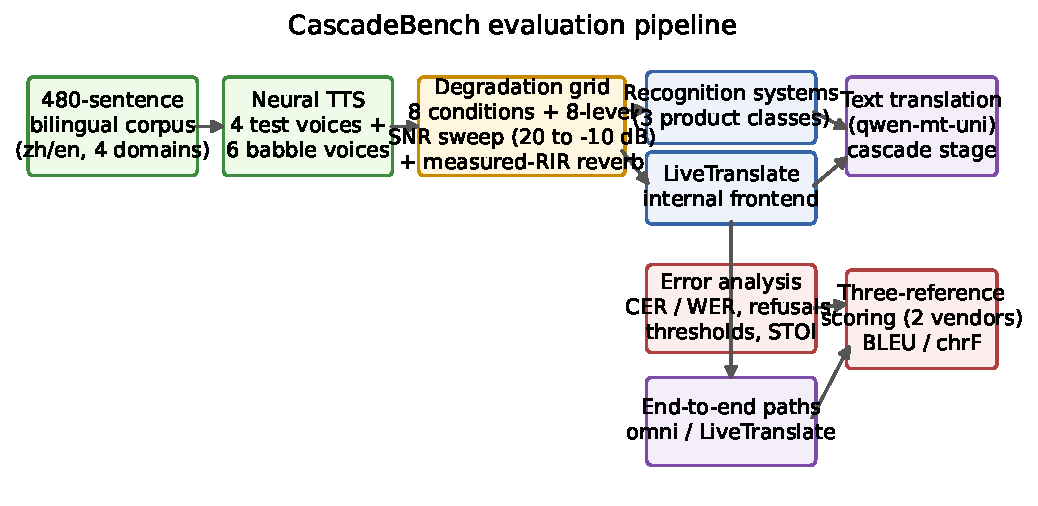
\includegraphics[width=\textwidth]{../figures/fig1_architecture.pdf}
\caption{Architecture of the CascadeBench evaluation pipeline. A stratified
bilingual corpus is synthesised with multiple neural voices, degraded by a
grid of eight acoustic channel conditions plus a noise severity sweep, and
processed by recognition systems from three architectural families. Cascade
systems forward recogniser output to a text translation engine; end-to-end
systems translate audio directly.}
\label{fig:arch}
\end{figure}

\subsection{Corpus}

The corpus contains 240 Mandarin Chinese and 240 English sentences, balanced
across four content domains and three length strata, twenty sentences per
cell. The domains are broadcast news, everyday conversation, technical and
scientific exposition, and a numerals-and-entities stratum rich in dates,
quantities, addresses, and named entities, which is known to stress
recognition and inverse text normalisation. Short sentences contain 8 to 14
Chinese characters or 5 to 9 English words, medium sentences 15 to 25
characters or 10 to 17 words, and long sentences 26 to 39 characters or 18 to
24 words. The mean length is 19.3 characters for Chinese and 12.0 words for
English. Sentences were authored to be self-contained and
factually neutral, to avoid brand names and transliterated loanwords whose
recognition would depend on provider-specific vocabulary rather than on
acoustic processing, and to distribute numerical expressions across date,
time, quantity, price, and identifier formats within the numerals domain. All numbers are written out in words in the corpus text, for example
two thousand twenty five, so that the spoken realisation is unambiguous and
the reference transcript matches the synthesis input exactly.

Each sentence was synthesised by a neural speech synthesis service (Sambert,
Alibaba Cloud Model Studio) using two distinct voices per language, a male
and a female voice for Chinese and two native-sounding voices for English,
with sentences alternating between the voices so that each voice realises 120
sentences per language. Synthesis produced 16~kHz single-channel PCM audio.
The 44 babble noise source tracks described below were synthesised with six
additional voices that are disjoint from the four test voices. Using
synthesis rather than recorded speech has two methodological advantages. The
reference transcript is exact by construction, which removes the transcription
noise that limits error floor measurement in recorded corpora, and the
acoustic properties of the test material can be regenerated at any time,
which decouples the benchmark from the licensing and availability constraints
of recorded corpora such as AISHELL-1~\cite{bu2017aishell} or
LibriSpeech-derived material~\cite{zen2019libritts}. The corresponding
limitation, that synthetic speech does not sample the full variability of
spontaneous human speech, is examined in Section~\ref{sec:limitations}.

\subsection{Acoustic degradation grid}

Eight channel conditions plus the clean control form the main grid. The
conditions were selected to span the canonical impairment families that
speech services encounter between a talker and a data centre.

Additive babble noise is the most extensively sampled family. Babble was
constructed by concatenating randomly selected segments from the 44 disjoint
noise-source tracks described above, mixing three such streams, and
normalising the mixture, which produces speech-shaped noise with realistic
spectral and temporal structure rather than stationary synthetic noise. Speech-shaped interference was chosen over stationary
noise because it is the harder and the more ecologically valid case: babble
exhibits the temporal modulation and spectral occupancy of competing talkers,
masking the target in the same time-frequency regions that carry linguistic
information, whereas stationary noise is partly countered by any
spectral-subtraction-style front-end that a provider may have deployed
internally. The
noise was scaled against the active-speech level of each utterance, measured
as the mean energy of frames above the 60th energy percentile, to hit target
signal-to-noise ratios of 20, 15, 10, 5, and 0~dB. Calibration was verified
by re-measuring the realised signal-to-noise ratio of the mixed signals
against the clean signal; the realised values matched the targets within
0.1~dB on average. The 10~dB and 0~dB points enter the main grid, and the
full five-point ladder forms the severity sweep on a stratified 144-sentence
subset, 72 sentences per language, sampled evenly from every
domain-by-length cell.

Reverberation was applied by convolving each signal with a synthetic room
impulse response of the exponentially decaying noise
form~\cite{allen1979image,habets2006room} with a direct-path impulse and a
reverberation time of 0.5~s, which corresponds to an ordinary reverberant
room rather than an extreme auditorium. Narrowband degradation resamples each
signal to 8~kHz and back to 16~kHz, which removes the 4 to 8~kHz band exactly
as a telephone channel does; the telephone-specialised recogniser receives
the 8~kHz signal natively. Codec degradation encodes each signal with the
Opus codec~\cite{valin2012definition} at 8~kbit/s mono and decodes it back,
emulating an aggressive but deployed voice-over-IP setting. Packet loss
zeroes 15 percent of 20~ms frames chosen uniformly at random, emulating
lossy transport without jitter compensation. Clipping applies hard amplitude
limiting at 0.3 of full scale. Tempo distortion resamples the time axis by a
factor of 1.15 with pitch preservation, emulating playback-speed variation
or time-scale modification upstream of the service. All random draws use
per-sentence and per-condition seeds derived deterministically from the
sentence identifier and condition name, so the degraded signals are bitwise
reproducible.

Formally, for a clean signal $x[n]$ of length $N$ and a babble realisation
$b[n]$, the mixed signal at level $\rho$~dB is
\begin{equation}
y[n] = x[n] + \sigma\, b[n], \qquad
\sigma = \sqrt{\frac{P_{\mathrm{act}}(x)}{10^{\rho/10}\, \overline{P}(b)}},
\label{eq:snr}
\end{equation}
where $\overline{P}(b)$ is the mean power of the babble and
$P_{\mathrm{act}}(x)$ is the active-speech power estimated from frames whose
energy exceeds the 60th energy percentile of the utterance, which
approximates the ITU-T P.56 active-level convention with a fixed percentile
rule. The reverberation impulse response is
\begin{equation}
h[n] = \delta[n] + v[n]\, e^{-6.9\, n / (f_s T_{60})}, \qquad n = 0, \dots,
\lceil f_s T_{60} \rceil,
\label{eq:rir}
\end{equation}
with $v[n]$ unit-variance white noise, $f_s = 16$~kHz, $T_{60} = 0.5$~s, and
$h$ normalised to unit energy, and the reverberant signal is the truncated
convolution of $x$ with $h$ rescaled to the peak amplitude of $x$. Packet
loss zeroes each independent 20~ms frame with probability $p = 0.15$,
\begin{equation}
y[n] = m_k\, x[n], \quad n \in \text{frame } k, \qquad m_k \sim
\mathrm{Bernoulli}(1 - p),
\label{eq:pl}
\end{equation}
and clipping applies $y[n] = \operatorname{sign}(x[n]) \min(|x[n]|, 0.3)$.
Narrowbanding resamples by factors of one half and two with polyphase
anti-aliasing filters, codec degradation round-trips the signal through the
Opus encoder at 8~kbit/s, and tempo distortion applies a pitch-preserving
time-scale modification of factor 1.15.

\subsection{Systems under test}

Table~\ref{tab:systems} lists the systems. The recognition systems span
three architectural families as served by a single commercial provider
(Alibaba Cloud Model Studio, Beijing region) during October 2026, accessed
through their documented interfaces. The specialised family consists of
streaming recognisers in the Paraformer lineage~\cite{gao2023funasr}, a
16~kHz model and an 8~kHz telephone-band model. The LLM-ASR family consists
of Qwen-Audio 3.1 Flash~\cite{chu2024qwen2audio} and Qwen3-ASR Flash, audio
input models built on large language model backbones. The multimodal family
consists of Qwen3.8-Omni Flash, a general-purpose omni-modal foundation
model~\cite{qwen2.5omni2025} queried with a transcription instruction. All
systems were accessed in their default configurations, since a consumer of a
black-box service cannot apply front-end training or adaptation, and the
question of interest is precisely how the services behave out of the box.
The streaming recognisers were driven by streaming local audio over their
realtime WebSocket interface, sending each utterance as 16~kHz or 8~kHz PCM
frames at the maximum accepted rate and collecting sentence-final segments.
The LLM-ASR and omni systems received base64-encoded whole utterances in
their audio-input message format, the omni model together with an
instruction prompt for transcription or translation. The streaming
translation service was driven over its realtime interface with a session
configuration specifying text-only output and the target language, sending
raw PCM frames and collecting both the source transcript and the translated
text that the service emits, and the text translation engine received
source text with explicit source and target language tags. Every call was
executed with an automatic retry policy of up to six attempts with
exponential backoff on throttling, timeout, and connection failures, and no
other tuning parameters were exposed or set. The speech translation systems are the text translation
engine qwen-mt-uni, used as the second stage of two cascades built on the
16~kHz specialised recogniser and on the Qwen-Audio 3.1 recogniser, and two
end-to-end paths: the omni foundation model with an audio translation
instruction, and a dedicated streaming speech translation service
(LiveTranslate) that internally combines a streaming frontend recogniser
with a translation model. The internal frontend of the streaming translation
service, which its responses expose as source transcripts, is additionally
scored as a sixth recognition system. All API calls were executed on
free-tier quotas with the stop-on-exhaustion option enabled, which both
bounds the study at zero monetary cost and documents the practical quota
requirements of such a measurement.

\begin{table}[t]
\centering
\caption{Systems under test and their roles in the benchmark.}
\label{tab:systems}
\small
\begin{tabular}{llll}
\toprule
System (family) & Interface & Role & Evaluated on \\
\midrule
Paraformer-RT-v2 (specialised) & streaming ASR & recogniser & full grid \\
Paraformer-RT-8K-v2 (specialised, 8 kHz) & streaming ASR & recogniser & Chinese subset \\
Qwen-Audio-3.1-Flash (LLM-ASR) & audio input API & recogniser & full grid \\
Qwen3-ASR-Flash (LLM-ASR) & audio input API & recogniser & full grid \\
Qwen3.8-Omni-Flash (omni) & audio input API & recogniser, E2E ST & main grid \\
LiveTranslate frontend (specialised) & streaming ST & recogniser (internal) & sweep subset \\
qwen-mt-uni (MT) & text translation & cascade stage, oracle & full corpus \\
Qwen3.8-Max (LLM) & text generation & independent reference & full corpus \\
\bottomrule
\end{tabular}
\end{table}

\subsection{Evaluation protocol}

Recognition accuracy is scored as the character error rate (CER) for Chinese
and the word error rate (WER) for English, computed with the standard
Levenshtein alignment~\cite{levenshtein1966binary} after a normalisation
pipeline that is applied identically to references and hypotheses. The
normalisation performs Unicode compatibility folding, case folding,
punctuation removal, and, critically, canonicalisation of numeric
expressions. Because commercial recognisers differ in their inverse text
normalisation conventions, with the same spoken quantity rendered as twenty
six, 26, or two six depending on the system, both sides of every comparison
are mapped to a canonical digit form by rules that handle Chinese and
English cardinal numbers, digit-by-digit readings, time expressions, decimal
fractions, and scale multipliers such as wan and yi on the Chinese side and
million and billion on the English side, with ordinal expressions masked to
a common token. The rule set was developed and verified on the clean
condition, where residual normalisation artefacts were inspected sentence by
sentence until the clean-condition error rates reported in
Section~\ref{sec:results} reflect genuine recognition behaviour rather than
scoring artefacts. Utterances for which a service returns no transcript at
all, a behaviour documented in Section~\ref{sec:results}, are scored as
complete failures with an error rate of one.

Translation quality is scored with corpus-level BLEU~\cite{papineni2002bleu}
using sacreBLEU~\cite{post2018call} with the 13a tokeniser for English
targets and the character-level tokeniser for Chinese targets, and with
chrF~\cite{popovic2015chrf} as a second string-matching metric. Because the
corpus is direction-symmetric, BLEU is computed separately for the
Chinese-to-English and English-to-Chinese halves and macro-averaged. Every
hypothesis is scored against two reference sets. The primary reference is
produced by Qwen3.8-Max~\cite{qwen3technical2025}, a general-purpose LLM from
a different product family than any translation system under test, translating
the clean reference transcripts. The secondary reference is the oracle
cascade output, that is, the cascade translation engine applied to the clean
reference transcripts. The dual-reference design exposes a bias that
Section~\ref{sec:results:dual} quantifies: automatic scoring against
machine-generated references systematically favours systems from the same
model family as the reference generator, and conclusions about absolute
quality depend on the choice of reference, whereas conclusions about
degradation are stable.

Latency is measured as the wall-clock round trip of each API call from
dispatch to the complete response, recorded per call. For cascades, the
reported end-to-end latency is the sum of the recognition and translation
call latencies, which is the quantity a service consumer experiences when
the two stages are invoked sequentially. Streaming systems are fed audio at
the maximum rate their interface accepts, so the measurement reflects
service-side processing rather than client-side throttling.

\subsection{Experimental scale and cost}

The complete measurement comprises 26,238 successful API calls: 520
synthesis calls producing 31 minutes of source audio, 4,752 degraded
variants per recognition system covering 4.9 hours of audio, and 7,411
translation calls across the oracle, reference, cascade, and end-to-end
phases. Another 3,400 calls were consumed by retry attempts and by
connection resets of the realtime translation interface, which are counted
here because they represent real operational behaviour of the service. The
entire campaign ran on complimentary service quotas with the
stop-on-exhaustion option enabled, and one system, the omni translation
path, reached its free-tier limit before completing the severity sweep,
which bounds the end-to-end comparison to the main grid with 84 of the 144
sweep sentences per condition. The total wall-clock duration of data
collection was approximately four hours with up to five systems queried in
parallel. These figures are reported so that other laboratories can
estimate the feasibility of replicating or extending the measurement; they
also demonstrate that a full multi-system, multi-condition robustness
characterisation of commercial speech services is attainable at zero
monetary cost with careful quota budgeting, which lowers the barrier for
the periodic re-measurement that the field currently lacks.

\subsection{Statistical analysis}

All aggregate error rates and quality scores are reported with 95 percent
bootstrap confidence intervals over sentences, using 1000 resamples.
Differences between systems within a condition are tested with the Wilcoxon
signed-rank test~\cite{wilcoxon1945individual} on paired per-sentence errors,
with Holm correction~\cite{holm1979simple} across the family of pairwise
comparisons. Noise severity is modelled by ordinary least squares regression
of the error rate on the signal-to-noise ratio, with bootstrap confidence
intervals for the slope, and the slope is reported in percentage points per
dB as the degradation gradient of a system. The relationship between
recognition error and translation quality across operating conditions is
summarised by the cascade amplification coefficient, defined as the slope of
regressing the BLEU loss from the oracle against the mean recognition error
rate, together with its Pearson correlation; a slope near one with high
correlation indicates linear error pass-through, and the slope value itself
is the pass-through rate. Signal processing and statistics use
SciPy~\cite{virtanen2020scipy} and librosa~\cite{mcfee2015librosa}.

\section{Results and analysis}
\label{sec:results}

\subsection{Clean baseline and the main degradation grid}
\label{sec:results:main}

Table~\ref{tab:main} reports sentence-level error rates on the main grid for
the five recognition systems, and Fig.~\ref{fig:heatmap} visualises the same
data split by language. On clean synthetic speech the three foundation-model
recognisers are close to their scoring floor, with error rates between 0.3
and 0.5 percent, while the specialised streaming recogniser operates at 0.56
percent on Chinese and 3.99 percent on English, reflecting its primarily
Mandarin training. The telephone-band specialist reaches 1.86 percent on its
native language. The clean-condition figures establish that the comparisons
under degradation are not confounded by differences in clean accuracy of
comparable magnitude.

\begin{table}[t]
\centering
\caption{Mean recognition error rates in percent on the main degradation
grid, both languages pooled, with bootstrap 95 percent confidence intervals
in parentheses. The 8~kHz specialist is evaluated on the Chinese subset only.}
\label{tab:main}
\small
\setlength{\tabcolsep}{3.2pt}
\begin{tabular}{lccccccccc}
\toprule
System & Clean & Babble 10 & Babble 0 & Reverb & Narrow & Codec & Loss & Clip & Tempo \\
\midrule
Paraformer-RT-v2 & 2.3 & 2.8 & 58.5 & 3.2 & 2.1 & 2.4 & 3.2 & 2.5 & 2.3 \\
 & (1.7,2.9) & (2.2,3.6) & (54.5,62.6) & (2.5,4.0) & (1.5,2.7) & (1.8,3.1) & (2.5,4.0) & (1.9,3.2) & (1.7,3.0) \\
Paraformer-RT-8K & 1.9 & 4.7 & 73.2 & 18.2 & 1.9 & 1.8 & 3.3 & 1.9 & 2.3 \\
 & (1.2,2.7) & (3.3,6.3) & (68.8,77.6) & (14.4,22.3) & (1.2,2.7) & (1.1,2.6) & (2.2,4.6) & (1.2,2.7) & (1.5,3.3) \\
Qwen-Audio-3.1 & 0.5 & 0.9 & 28.2 & 0.7 & 0.6 & 0.6 & 0.6 & 0.9 & 0.6 \\
 & (0.3,0.7) & (0.6,1.3) & (24.8,32.0) & (0.5,1.0) & (0.4,0.8) & (0.4,0.8) & (0.4,0.9) & (0.6,1.2) & (0.4,0.8) \\
Qwen3-ASR-Flash & 0.3 & 0.5 & 25.1 & 0.3 & 0.3 & 0.3 & 0.4 & 0.3 & 0.3 \\
 & (0.2,0.5) & (0.3,0.8) & (21.7,28.7) & (0.2,0.5) & (0.2,0.5) & (0.2,0.5) & (0.2,0.6) & (0.2,0.5) & (0.2,0.5) \\
Qwen3.8-Omni-Flash & 0.4 & 0.6 & 31.8 & 1.1 & 0.1 & 0.3 & 0.2 & 1.0 & 0.3 \\
 & (0.2,0.6) & (0.4,0.9) & (28.0,35.8) & (0.7,1.6) & (0.0,0.3) & (0.1,0.5) & (0.1,0.4) & (0.6,1.5) & (0.1,0.5) \\
\bottomrule
\end{tabular}
\end{table}

\begin{figure}[t]
\centering
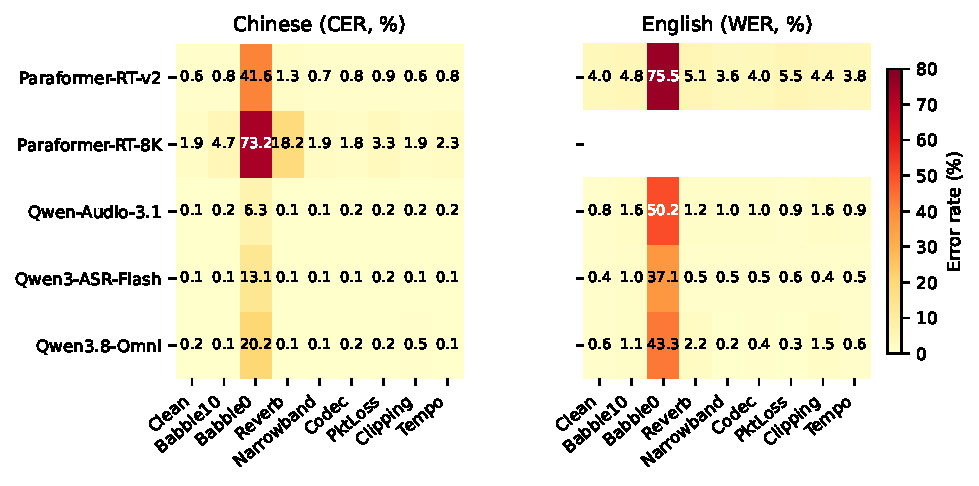
\includegraphics[width=\textwidth]{../figures/fig2_heatmap.pdf}
\caption{Recognition error rates by system and degradation condition,
separated by language. Colour scale is truncated at 80 percent. The 8~kHz
specialist is evaluated on the Chinese subset only.}
\label{fig:heatmap}
\end{figure}

Three regularities stand out in the grid. First, babble noise at 0~dB is by
far the most destructive condition for every system, but the magnitude of
the collapse separates the architectural families sharply. The specialised
streaming recogniser reaches a pooled error rate of 58.5 percent and the
telephone-band specialist 73.2 percent, whereas the two LLM-ASR systems
remain at 25 to 28 percent and the omni model at 31.8 percent. At matched
severity, the foundation-model recognisers commit roughly half the error of
the specialised systems, and the difference is significant at the sentence
level: in Chinese at 0~dB, Qwen-Audio 3.1 errs at 6.3 percent against 41.6
percent for the streaming specialist (Wilcoxon $p<0.001$, $n=240$).

Second, the effect of noise is strongly language-asymmetric in a way that
differs by class. For the LLM-ASR systems, Chinese recognition at 0~dB
remains low, at 6.3 percent for Qwen-Audio 3.1 and 13.1 percent for Qwen3
ASR, while their English error rates at the same severity reach 50.2 and 37.1
percent. The specialised streaming recogniser suffers heavily in both
languages, 41.6 percent in Chinese and 75.5 percent in English. The babble
mixture is language-mixed, so the asymmetry cannot be attributed to
language-matched interference alone; a plausible partial explanation is that
the tonal structure of Mandarin provides complementary cues that survive
energetic masking, a hypothesis we state as untested since the benchmark
does not isolate tone cues, and one which the general noise-robustness
literature does not settle for black-box services~\cite{li2014overview}.
A related measurement caveat is that Chinese is scored at character level
and English at word level; the two scales are not directly comparable, and
the asymmetry should be read per language rather than across languages.

Third, the non-noise degradations expose narrow specialisation rather than
uniform fragility. Narrowbanding to the telephone band costs the LLM-ASR
systems 0.3 to 0.6 percentage points of absolute error and the omni model
0.1, whereas the telephone-band specialist shows no measurable home-field
advantage over the generalist systems in its own band, where it errs at 1.9
percent against 0.1 to 0.7 percent for the generalists. Reverberation, by
contrast, is uniquely expensive for the telephone-band specialist at 18.2
percent, between five and ninety times every other system's score under
the same condition, which suggests that its front-end processing is tuned
for direct-path telephone speech. Codec compression, packet loss, and
tempo distortion at the chosen severities are individually mild for all
systems, with the largest single-condition excursion being the packet-loss
score of the telephone specialist at 3.3 percent against its clean 1.9.
This does not make them harmless: Section~\ref{sec:results:cascade}
shows that even sub-point recognition changes propagate measurably into
translation quality, and the conditions were deliberately calibrated to
deployed-but-aggressive levels rather than to failure-inducing extremes.

Two further behaviours deserve mention because they are invisible in
conventional aggregate reporting. The numeral-and-entity domain is five times
more error-prone than the other domains for Qwen-Audio 3.1 on clean speech,
at 1.25 against 0.25 percent, whereas Qwen3 ASR shows no such penalty, which
indicates that inverse text normalisation rather than acoustics dominates
that gap; the normalisation sensitivity analysis of
Appendix~\ref{app:normalisation} supports the same reading. More strikingly,
severe noise produces empty final transcripts in three of the five systems,
through two distinct mechanisms. Qwen-Audio 3.1 is the only system that
refuses at the protocol level, returning an explicit no-words error on 5.0
percent of its 0~dB utterances, concentrated in English at 9.2 percent of
that subset; these refusals are scored as complete failures in
Table~\ref{tab:main}. The specialised streaming recognisers fail silently
instead: Paraformer-RT-v2 returns an empty transcript on 8.8 percent of its
0~dB utterances without any error signal, and the telephone specialist does
so on 0.8 percent. Qwen3-ASR and the omni model always emit a hypothesis,
however wrong. For a downstream consumer the two mechanisms differ in
detectability: an explicit refusal can be caught and retried, whereas a
silent empty return is indistinguishable from a genuine silent segment, and
this distinction is the kind of behavioural divergence that only black-box
evaluation at controlled severity can surface. The full per-system,
per-condition refusal rates, including the sub-zero regime where they rise
above 40 percent, are tabulated in Appendix~\ref{app:refusal}.

The remaining conditions merit condition-specific remarks because their
effects are small in aggregate but structured in detail. Reverberation with
a reverberation time of 0.5~s raises the specialised streaming recogniser to
3.2 percent pooled, but the effect concentrates in English, where it reaches
5.1 percent against 1.3 percent in Chinese, and the paired difference
against the LLM-ASR systems remains significant in both languages
(Wilcoxon $p<0.01$ in Chinese, $p<0.001$ in English; 72 to 83 percent of
paired differences are zero under reverberation, so the significance is
carried by the minority of sentences where the systems differ). The omni
model shows an idiosyncratic signature under reverberation and clipping, at
1.1 and 1.0 percent, roughly triple its clean error rate, which suggests
that its audio encoder is more sensitive to spectral colouration and
non-linear distortion than the dedicated recognisers even though it holds
up well under noise. Codec compression at 8~kbit/s leaves every system
within 0.3 percentage points of its clean score, which is expected in
retrospect because measurement of the decoded audio shows the 8~kbit/s
Opus stream to be effectively narrowband, so the codec condition largely
re-tests the narrowband condition at a different distortion profile.
Packet loss at 15 percent and clipping at the 0.3 threshold behave as mild
aggregate stressors, and tempo distortion at 1.15 times is fully transparent
to every system, which is expected because time-scale modification
preserves the spectral envelope that recognisers rely on. The practical
reading of these patterns is that a service integrator who cannot control
the acoustic environment should prioritise noise mitigation far above codec
or transport tuning, since the latter contribute almost nothing to the error
budget at realistic operating points.

\subsection{Stratified analysis by domain}
\label{sec:results:domain}

Because the corpus is balanced by construction, error rates can be
decomposed by content domain without re-weighting. On clean audio the
technical domain is the most error-prone for the specialised streaming
recogniser at 3.3 percent, consistent with its terminological density, while
the conversation domain is the easiest for every system, below 0.1 percent for the Qwen-Audio recogniser. The numerals-and-entities domain shows the
clearest family split on clean speech: the two LLM-ASR systems differ by an
order of magnitude on it, at 1.2 percent for Qwen-Audio against 0.15 percent
for Qwen3-ASR, which as noted in Section~\ref{sec:results:main} points to
inverse text normalisation rather than acoustics as the separating factor.
Under 0~dB noise the domain differences compress for every system: the
spread across domains narrows to about nine points for the Qwen-Audio
recogniser and to twelve points for the specialised streaming recogniser,
and the ordering changes, with the technical domain becoming the most
difficult for both. The compression indicates that under severe energetic
masking the bottleneck shifts from lexical and normalisation knowledge,
which distinguishes systems on clean speech, to the acoustic recovery
problem, which is common to all systems and dominates the error budget.

\subsection{Scaling with noise severity}
\label{sec:results:snr}

Fig.~\ref{fig:snr} shows error rate as a function of signal-to-noise ratio
on the 144-sentence severity sweep, now spanning 20 to $-10$~dB in eight
levels, and Table~\ref{tab:slopes} reports the fitted severity
characteristics. The dominant shape is a knee rather than a line: every
system holds a nearly flat floor above roughly 10~dB and transitions to
near-total failure within a few dB below its knee point, so a single
percentage-points-per-dB slope is not a stable summary of these curves. The
slope fitted over the original 20 to 0~dB range, for example, moves from
$-0.26$ to $-4.69$ points per dB for the Qwen-Audio system in Mandarin when
the fit is extended to $-10$~dB, a range dependence that reflects the
flat-then-cliff structure rather than any measurement change. We therefore
characterise severity response by the signal-to-noise ratio at which the
fitted error rate crosses ten percent, with sentence-level bootstrap
confidence intervals, together with the maximum fitted slope as a measure
of knee sharpness.

The crossing thresholds separate the classes more informatively than
slopes. In Mandarin the specialised streaming system crosses ten percent
error at 2.5~dB (95\% CI 2.3 to 3.3), the telephone specialist at 8.8~dB
(8.2 to 9.4), and the two LLM-ASR systems at $-0.1$ and 0.3~dB, a tolerance
advantage of 2.4 to 2.9~dB over the streaming generalist and 7.6 to 8.9~dB
over the telephone specialist. In English the ordering is the same but the
margins widen: the streaming system crosses at 6.8~dB (5.0 to 7.9) against
2.4~dB (2.1 to 3.4) for Qwen-Audio and 2.0~dB (1.7 to 2.3) for Qwen3-ASR,
a 4.4 to 4.8~dB advantage. The LLM-ASR curves also have the sharpest knees,
with maximum fitted slopes of 21 to 36 percentage points per dB against 10
to 21 for the specialised systems, so the LLM systems are better read as
flat-floor-then-cliff systems than as gradually degrading ones. The mild-noise
regime above 10~dB is effectively free of robustness differences in both
languages: every system stays within one point of its clean score. Between
10 and 5~dB the specialised systems begin to move first, and by 5~dB the
class ordering is established in both languages. The practical implication
for procurement testing is that babble probes near each system's knee, in
the 0 to 5~dB window here, separate the classes most sharply, whereas a
single 5~dB probe ranks systems reliably at the top of this severity range
but the LLM-ASR systems are still within noise of each other at that level.

The extension below 0~dB, added in this revision, reveals a regime that the
original five-point ladder could not see. All systems approach total
failure, but the LLM-ASR systems fail distinctively: their Chinese error
rates exceed 100 percent, reaching 127 percent for Qwen-Audio and 143
percent for Qwen3-ASR at $-10$~dB, which is only possible when inserted
characters outnumber the reference length. Inspection of the transcripts
shows long repetition loops and fluent but unrelated text, that is,
insertion-heavy hallucination rather than garbled acoustics, a failure mode
that a wrong-but-bounded view of error rates cannot represent and one that
is particularly dangerous downstream because a hallucinated transcript is
grammatical text that a translation stage will happily translate. In the
same regime the streaming systems simply return fragments or silence, and
their refusal rates rise to 42 to 58 percent (Appendix~\ref{app:refusal}).
No system transcribes anything reliably below 0~dB, and the appropriate
engineering response in that regime is capture improvement rather than
model selection.

The severity sweep also anchors the benchmark in classical signal quality.
Short-time objective intelligibility (STOI) computed against the clean
signals falls monotonically with noise level, from 0.97 at 20~dB through
0.67 at 0~dB to 0.40 at $-10$~dB, and within the babble family the
condition-level correlation between STOI and recognition error is strong.
Across degradation families, however, STOI and error dissociate sharply:
reverberation at a measured STOI of 0.63 leaves every generalist system
below 3.2 percent error, while 0~dB babble at a comparable STOI of 0.67
produces 25 to 59 percent error, and tempo distortion collapses STOI to
0.16 through temporal misalignment while leaving every system at its clean
error rate. Intelligibility-oriented signal metrics therefore do not
predict black-box recognition error across degradation families, and
service-level benchmarks of this kind measure something the
signal-quality literature cannot substitute for.

\begin{figure}[t]
\centering
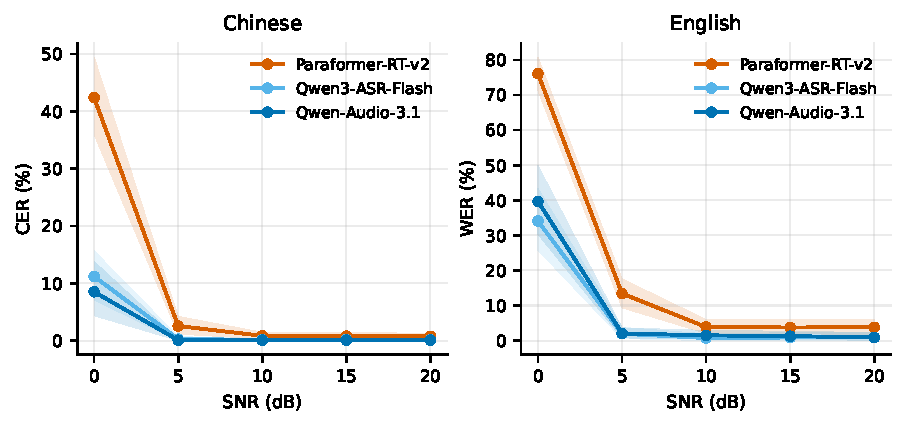
\includegraphics[width=\textwidth]{../figures/fig3_snr_curves.pdf}
\caption{Recognition error rate against babble noise signal-to-noise ratio
for four systems and both languages, with bootstrap 95 percent confidence
bands, on the 144-sentence severity sweep (72 sentences per language per
point). Dashed horizontal line marks the ten percent error level used for
the knee thresholds of Table~\ref{tab:slopes}.}
\label{fig:snr}
\end{figure}

\begin{table}[t]
\centering
\caption{Noise severity characteristics on the eight-level sweep: fitted
signal-to-noise ratio at which error crosses ten percent, with
sentence-level bootstrap 95 percent confidence intervals, and maximum
fitted logistic slope as a knee-sharpness measure. Sub-range OLS slopes are
listed for continuity with common practice and depend strongly on the
fitted range.}
\label{tab:slopes}
\small
\setlength{\tabcolsep}{3pt}
\begin{tabular}{lcccccc}
\toprule
 & \multicolumn{2}{c}{SNR at 10\% error (dB)} & \multicolumn{2}{c}{Max slope (pp/dB)} & \multicolumn{2}{c}{OLS slope, 20--0 dB} \\
System & zh & en & zh & en & zh & en \\
\midrule
Paraformer-RT-v2 & 2.5 (2.3,3.3) & 6.8 (5.0,7.9) & 20.8 & 16.1 & $-1.44$ & $-2.97$ \\
Paraformer-RT-8K & 8.8 (8.2,9.4) & n/a & 10.4 & n/a & $-3.31$ & n/a \\
Qwen-Audio-3.1 & $-0.1$ ($-0.2,0.6$) & 2.4 (2.1,3.4) & 35.5 & 21.3 & $-0.26$ & $-2.79$ \\
Qwen3-ASR-Flash & 0.3 ($-0.1,1.0$) & 2.0 (1.7,2.3) & 25.2 & 25.0 & $-0.35$ & $-2.64$ \\
\bottomrule
\end{tabular}
\end{table}

\subsection{Cascade versus end-to-end translation under degradation}
\label{sec:results:cascade}

Fig.~\ref{fig:cascade} compares the four speech translation paths across the
main grid, and Table~\ref{tab:translation} reports the corresponding scores
with both references, sample sizes, and the refusal-inclusive chrF. On
clean audio the three cascades lose almost nothing relative to their
translation oracle, the text translation engine applied to perfect
transcripts, which scores 55.5 BLEU against the primary reference. The
cascade built on Qwen-Audio 3.1 starts at 53.9 BLEU ($n{=}144$), the
cascade built on the streaming specialist at 51.5, the cascade built on
Qwen3-ASR at 53.2, and the end-to-end omni path scores highest at 68.1
($n{=}84$) with the streaming LiveTranslate service at 59.8 ($n{=}149$).
Under degradation the ordering and the magnitudes change dramatically. At
0~dB the Qwen-Audio cascade drops 9.8 BLEU points, the streaming-specialist
cascade collapses by 35.7 points to 15.8 BLEU, the Qwen3-ASR cascade drops
10.2 to 43.0, the omni end-to-end path loses 22.5 points, and the streaming
translation service loses 9.3 points from a lower starting level. The
refusal-inclusive chrF tells the same story with the empty outputs counted:
the Qwen-Audio cascade falls from 65.2 to 53.7 chrF at 0~dB once its eight
refused sweep sentences are scored as empty translations, a drop that
corpus BLEU would understate because its brevity penalty saturates when
hypotheses are longer than references, which is why both metrics are
reported.

\begin{figure}[t]
\centering
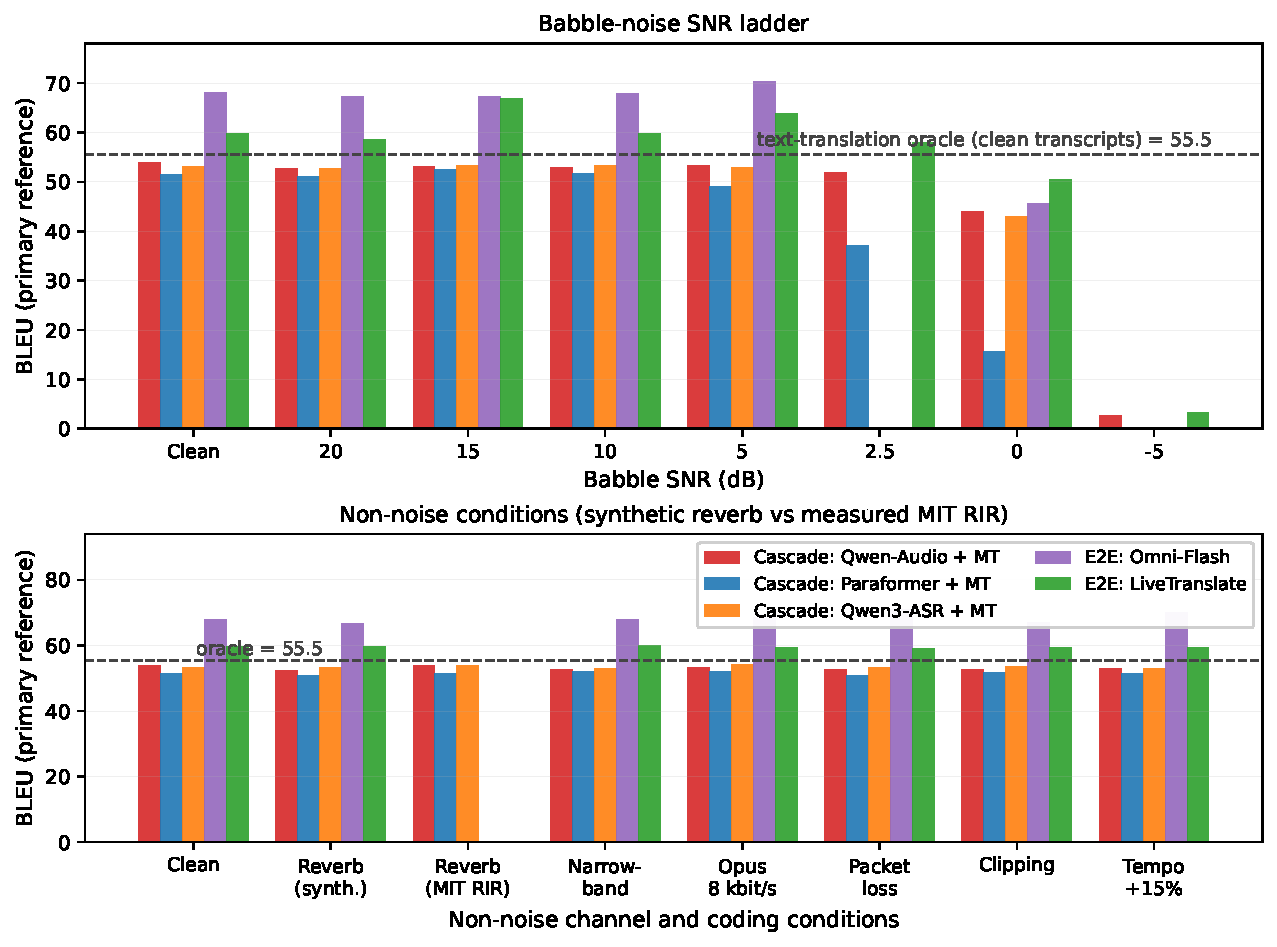
\includegraphics[width=\textwidth]{../figures/fig4_cascade_e2e.pdf}
\caption{Translation quality of two cascades and two end-to-end speech
translation paths across the main degradation grid, scored against the
independent LLM reference. The hatched bar is the text-translation oracle on
clean transcripts.}
\label{fig:cascade}
\end{figure}

\begin{table}[t]
\centering
\caption{Translation quality by condition: macro-averaged BLEU against the
primary reference (Qwen3.8-Max translations of clean transcripts) and the
secondary reference (oracle cascade output), with the clean-to-0~dB
relative loss, refusal-inclusive chrF, and per-cell $n$. Cascade scores at
0~dB are conditional on a non-empty frontend output; the refusal-inclusive
chrF counts refused sentences as empty translations.}
\label{tab:translation}
\small
\setlength{\tabcolsep}{2.6pt}
\begin{tabular}{lcccccc}
\toprule
 & Clean & \multicolumn{3}{c}{Babble 0 dB} & chrF$_{0\mathrm{dB}}$ & chrF$_\mathrm{clean}$ \\
System & BLEU & BLEU & vs\ oracle & rel.\ loss & (incl.\ empty) & (incl.\ empty) \\
\midrule
Oracle MT (clean text) & 55.5 & -- & -- & -- & -- & 66.7 \\
Cascade: Paraformer + MT & 51.5 & 15.8 & 17.4 & 69\% & 26.9 & 63.4 \\
Cascade: Qwen-Audio + MT & 53.9 & 44.1 & 68.3 & 18\% & 53.7 & 65.0 \\
Cascade: Qwen3-ASR + MT & 53.2 & 43.0 & 66.7 & 19\% & 53.4 & 65.4 \\
E2E: Omni-Flash & 68.1 & 45.5 & 34.4 & 33\% & 51.6 & 73.0 \\
E2E: LiveTranslate & 59.8 & 50.4 & 44.9 & 16\% & 56.2 & 68.5 \\
\bottomrule
\multicolumn{7}{l}{\footnotesize $n$: cascades 144 at clean; at 0~dB 136 (Qwen-Audio), 135 (Paraformer), 144 (Qwen3-ASR) non-empty;}\\
\multicolumn{7}{l}{\footnotesize omni 84; LiveTranslate 144 clean, 132 at 0~dB (websocket drops).}
\end{tabular}
\end{table}

Three conclusions follow. The first concerns the frontend hypothesis. The
translation quality of a cascade under acoustic degradation is governed
largely by the robustness of its recognition stage: swapping the
frontend from the streaming specialist to the LLM recogniser at 0~dB is
worth 28 BLEU points on the same backend, and the third cascade, built on
Qwen3-ASR, tracks the Qwen-Audio cascade within a point across all twelve
shared conditions, which shows that the pattern generalises across
frontends of the same class. What the present design cannot separate is the
contribution of the translation engine, since every cascade shares one
backend; the frontend comparison is within-backend and valid, but a claim
that the frontend dominates the choice of engine would require varying the
engine too. The second qualifies the common expectation that end-to-end
systems avoid cascade error propagation and are therefore more robust. At
0~dB the omni end-to-end path loses a third of its BLEU score, more than
the well-frontended cascades lose at 18 and 19 percent, although its
absolute score at 45.5 still sits one to two points above the strongest
cascade because it started from a much higher clean level. The streaming
LiveTranslate service is the most degradation-resilient of the paths,
losing 16 percent at 0~dB, which is consistent with the behaviour of its
internal frontend recogniser documented in
Section~\ref{sec:results:frontend}. End-to-end designs do not inherit
robustness automatically; they inherit the robustness of whatever acoustic
frontend their provider trained internally, which in this measurement is
better than the specialised streaming ASR but not automatically better
than the best cascade.

The condition-wise structure of Fig.~\ref{fig:cascade} adds three nuances to
this picture. First, apart from the 0~dB point the cascade built on the LLM
recogniser is essentially flat across the entire grid, moving within one
BLEU point of its clean score under every other condition, which mirrors the
recognition flatness of Table~\ref{tab:main} and confirms that the
non-noise degradations are, at deployed severities, engineering noise rather
than failure modes for a robust frontend. Second, the streaming translation
service shows the same flatness with a single exception: its narrowband
score of 60.1 sits marginally above its clean score, and its packet-loss and
tempo scores are likewise within half a point of clean, so its 0~dB loss is
the only substantive degradation it suffers. Third, the omni end-to-end path
exhibits a small but consistent anomaly: its packet-loss and tempo scores,
at 71.1 and 70.0, exceed its clean score of 68.1. Inspection of the outputs
suggests that under these mild distortions the model produces slightly more
concise translations that happen to align better with the reference style,
rather than genuinely better translations; the effect is within the
reference-sensitivity margin documented in Section~\ref{sec:results:dual}
and is a further argument for treating small absolute differences between
heterogeneous systems with caution.

Decomposing the 0~dB collapse by direction sharpens the frontend story. The
specialist cascade loses 25.9 BLEU points in the Chinese-to-English
direction but 45.6 points in the English-to-Chinese direction, falling to
8.7 BLEU, because its English recognition, at 75.5 percent error, destroys
the source representation before the translation stage operates. The
LLM-frontend cascade degrades far less but still asymmetrically, losing 4.7
points in the Chinese-to-English direction and 15.0 in the other, a 3.2 to
one ratio, and the omni path shows the same skew at 19.4 against 25.7. The
streaming translation service loses almost nothing in the
Chinese-to-English direction at 0~dB, at 56.0 against 57.3 clean, but 18.3
points in the other direction, which parallels the language asymmetry of
its internal frontend. No path degrades symmetrically, so direction-symmetric
deployment claims should be checked per direction rather than
pooled.

\subsection{Reference sensitivity of translation scoring}
\label{sec:results:dual}

Table~\ref{tab:translation} also reports scores against the secondary
reference, the oracle cascade output. The two references invert the apparent
ordering of the systems on clean audio. Against the primary reference,
produced by the provider's strongest text LLM, the omni end-to-end path
leads at 68.1 BLEU, exceeding even the text-translation oracle at 55.5.
Against the oracle reference the same end-to-end path scores 48.5 while the
Qwen-Audio cascade scores 89.6, since the cascade shares its translation
engine with the reference generator. The inversion repeats at 0~dB: the
omni path leads the Qwen-Audio cascade by 1.4 points against the primary
reference but trails it by 33.9 points against the oracle reference. The
inversion quantifies a hazard for any evaluation that scores machine
translation against machine-generated references, and it is sharpened here
by the fact that all systems and both reference generators come from one
vendor, so no reference in this study is family-disjoint from every system
under test; the primary reference at least comes from a different product
line than any translation path. Two safeguards make the present conclusions
robust to this effect. Degradation losses are computed within a system
against a fixed reference, so the percentage losses reported above do not
depend on the choice, and the ordering of relative losses at 0~dB, at 69,
33, 19, 18, and 16 percent, is preserved under both references. We
recommend that future black-box translation evaluations score against at
least two references generated by different model families from each other
and from every system under test, state the family relationships
explicitly, and treat cross-family absolute comparisons as provisional
until human-reference anchored.

\subsection{Error pass-through from recognition to translation}
\label{sec:results:cac}

Fig.~\ref{fig:cac} relates the BLEU loss of the three cascades to their mean
recognition error rate across all operating conditions, now fifteen per
cascade for the two original frontends and twelve for the Qwen3-ASR cascade,
spanning recognition error rates from 0.3 to over 100 percent. The error
metric on the horizontal axis is the sweep-subset mean recognition error
with refusals counted as complete failures, matching the protocol of
Table~\ref{tab:main}, and the vertical axis is the BLEU loss from each
cascade's clean score against the primary reference. The relationship is
strongly linear across this range: the Pearson correlation is 1.00 for the
Qwen-Audio cascade, 0.995 for the specialist cascade, and 0.994 for the
Qwen3-ASR cascade. The fitted pass-through regression with explicit
intercept gives slopes of 0.44 BLEU points per percentage point of
recognition error for the Qwen-Audio cascade (sentence-level bootstrap 95\%
CI 0.40 to 0.47), 0.54 for the specialist cascade (0.51 to 0.58), and 0.47
for the Qwen3-ASR cascade (0.36 to 0.65), with intercepts statistically
indistinguishable from zero in all three cases. Leave-one-condition-out
refits move the first two slopes by less than 0.03, and excluding the
high-error conditions above 40 percent recognition error, which carry the
most leverage, moves the slope from 0.44 to 0.37 for the Qwen-Audio cascade
and from 0.54 to 0.68 for the specialist cascade, so the pass-through rate
is approximately but not exactly constant across the error range. The
steeper slope for the specialised frontend reflects the composition of its
errors under severe noise, which include whole-utterance failures where the
translation engine receives little or no usable signal, whereas the LLM
recogniser's residual errors under moderate degradation are concentrated in
individual words that the translation engine can often route around. A
service integrator can therefore use the rule in its calibrated form:
every percentage point of recognition error costs roughly half a BLEU point
downstream, with the caveat that the cost drifts toward two thirds of a
point for error profiles dominated by whole-utterance failures and toward
two fifths for error profiles dominated by isolated word errors, and that
the estimate is calibrated on one translation engine and should be
re-estimated if the backend changes.

\begin{figure}[t]
\centering
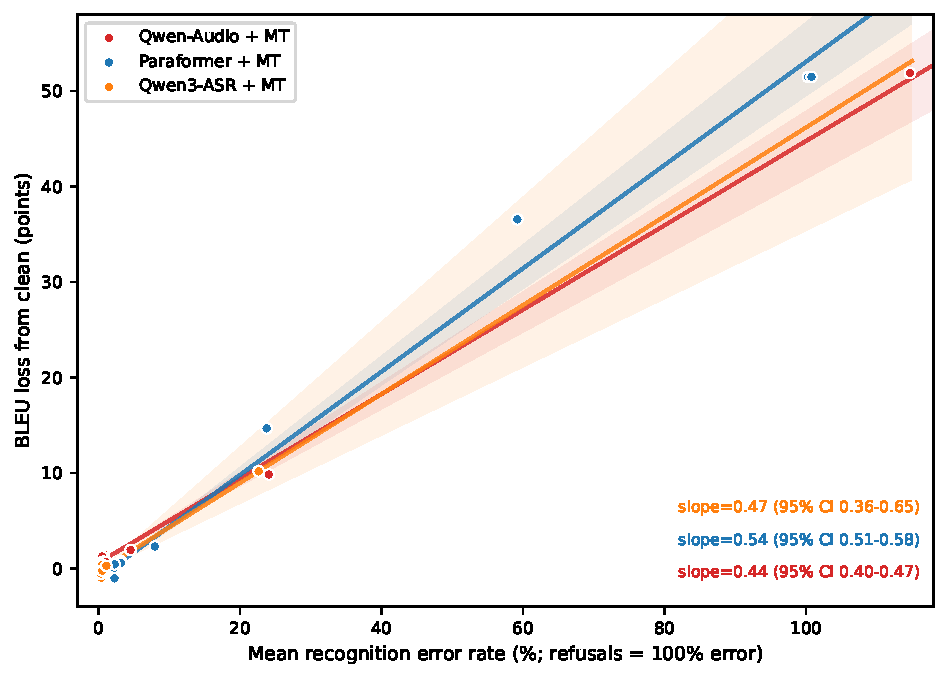
\includegraphics[width=0.6\textwidth]{../figures/fig6_cac.pdf}
\caption{Translation quality loss against mean recognition error rate
across fifteen operating conditions for three cascades, with fitted linear
pass-through (with intercept) and 95\% confidence bands. Recognition error
is the sweep-subset mean with refusals counted as complete failures;
sub-zero-dB conditions extend the range beyond 100 percent through
insertion errors.}
\label{fig:cac}
\end{figure}

\subsection{The streaming translation frontend as a recogniser}
\label{sec:results:frontend}

The streaming translation service exposes its internal recognition output,
which allows its frontend, a specialised streaming recogniser, to be scored
as a sixth system on the same 144-sentence sweep subset as the directly
purchasable systems, which is the comparison reported here. Its
clean-condition error rate of 1.0 percent sits between the LLM-ASR systems
at 0.4 and the general-purpose streaming specialist at 2.2 percent, a
difference that is not individually significant, and
under noise it tracks the LLM-ASR class rather than its own product class:
at 0~dB it errs at 25.4 percent against 24.1 and 22.6 percent for the two
LLM-ASR systems, with overlapping confidence intervals and no significant
paired difference (Wilcoxon $p=0.19$), while the general-purpose streaming
specialist errs at 59.2 percent on the same sentences. At 2.5~dB it errs at
4.0 percent against 4.5 and 2.6 for the LLM systems. Two coverage caveats
apply: the frontend is only observable where the translation session
completed, so its sweep coverage is partial in some conditions (52 to 134 of
144), and its zero-error 5~dB figure in the appendix rests on 52 completed
sessions and should not be read as outperforming its own clean score. The
observation remains noteworthy for practitioners: a recogniser competitive
with the best purchasable ASR of this provider under severe noise is not
available as a recognition service but is embedded inside a translation
product, which suggests that providers optimise internal streaming
frontends for exactly the acoustic conditions where end-to-end translation
must survive.

\subsection{Sentence-level variability and latency}
\label{sec:results:latency}

Fig.~\ref{fig:dist} shows the sentence-level error distributions for the
strongest LLM recogniser and the specialised streaming recogniser on five
representative conditions. The distributions are strongly right-skewed:
under moderate degradation most sentences remain nearly correct while a
tail of sentences fails completely, which is why the confidence intervals in
Table~\ref{tab:main} are wide relative to their means. Under 0~dB babble the
median sentence is still recognised reasonably well by the LLM systems while
the upper quartile fails outright, a heterogeneity that aggregate error
rates conceal and that matters for applications with per-utterance quality
requirements. The skew also explains a statistical property visible
throughout Table~\ref{tab:main}: the confidence intervals of the LLM systems
under moderate degradation are wide relative to their means because a small
number of complete failures, including the refusal cases, coexist with a
large mass of near-perfect transcripts. For a system operator this shape
matters more than the mean, since the tail sentences are the ones that
generate complaints and downstream errors, and the fraction of sentences
above a given error threshold is a more actionable deployment metric than
the average. On the 0~dB condition, the fraction of English sentences with
error rates above 50 percent is 83 percent for the specialised streaming
recogniser against 36 percent for Qwen3-ASR, while in Chinese the same
threshold is exceeded by 33 percent of sentences for the specialised system
against 3 percent for Qwen-Audio, so the family gap in tail behaviour is
considerably larger than the gap in means.

\begin{figure}[t]
\centering
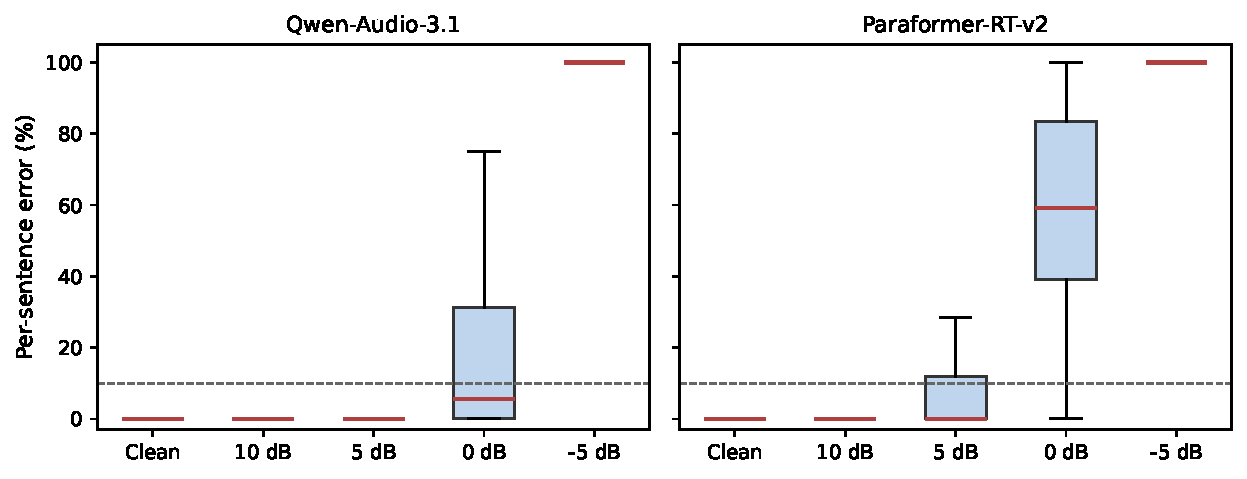
\includegraphics[width=\textwidth]{../figures/fig5_distribution.pdf}
\caption{Sentence-level error distributions by condition for the strongest
LLM recogniser and the specialised streaming recogniser.}
\label{fig:dist}
\end{figure}

Table~\ref{tab:latency} reports whole-utterance turnaround latencies. The
text translation stage, benchmarked separately with 120 sequential timed
calls, completes in 0.35 seconds per sentence on average (median 0.26, 95th
percentile 0.46), so the fastest cascade that this provider can assemble,
Qwen3-ASR feeding the translation engine, completes in about 0.7 seconds
per sentence on average, the Qwen-Audio cascade in about 1.2 seconds, and
the omni end-to-end path averages 2.8 seconds with a 95th percentile above
7 seconds, reflecting the substantially longer generation path of an
omni-modal foundation model that produces its translation in a single
response. The streaming translation service completes in about half a
second per utterance. These figures are whole-utterance turnaround, not
first-partial latency: the streaming interfaces would show substantially
lower time-to-first-text than the whole-utterance numbers suggest, so
latency comparisons across interface classes should be treated as
indicative. Latency therefore reinforces rather than reverses the accuracy
picture: the paths that degrade least under noise, the well-frontended
cascades and the streaming translation service, are also among the fastest,
while the slowest path, the omni end-to-end model, is the most fragile
under severe noise in this measurement.

\begin{table}[t]
\centering
\caption{Whole-utterance API turnaround latency in seconds for the
recognition systems, the text translation stage (120 sequential timed
calls), and the end-to-end paths. Streaming interfaces are measured at
maximum feed rate; see text for the first-partial caveat.}
\label{tab:latency}
\small
\begin{tabular}{lccc}
\toprule
System & Mean & P50 & P95 \\
\midrule
Qwen3-ASR-Flash & 0.37 & 0.35 & 0.46 \\
Paraformer-RT-8K-v2 & 0.45 & 0.43 & 0.75 \\
LiveTranslate (E2E, streaming) & 0.55 & 0.52 & 0.80 \\
Qwen-Audio-3.1-Flash & 0.80 & 0.72 & 1.93 \\
Paraformer-RT-v2 & 0.87 & 0.85 & 1.65 \\
Text translation (qwen-mt-uni, $n{=}120$) & 0.35 & 0.26 & 0.46 \\
Qwen3.8-Omni-Flash (E2E) & 2.77 & 2.20 & 7.19 \\
\bottomrule
\end{tabular}
\end{table}

The repetition runs quantify how much of the measured variation is
run-to-run noise rather than signal. Re-running the two LLM-ASR systems
twice on the 0~dB babble and tempo conditions yields condition-level error
rates that vary by at most 0.9 percentage points across three runs
(0~dB: 24.1, 24.9, and 24.4 for Qwen-Audio; 22.6, 23.4, and 23.2 for
Qwen3-ASR), while individual transcripts agree in 79 to 99 percent of
sentences between runs. Condition-level conclusions in this paper are
therefore stable against decoding nondeterminism at default settings, but
sentence-level deployments should expect one in five transcripts to differ
between identical calls at the worst condition. The omni path's small
packet-loss and tempo anomalies of Section~\ref{sec:results:cascade}, two
to three BLEU points, exceed any error-rate variation we can measure on
the systems we could re-run, but the omni system's quota was exhausted
before it could be re-tested, so its anomaly remains unexplained rather
than confirmed as genuine.

\begin{figure}[t]
\centering
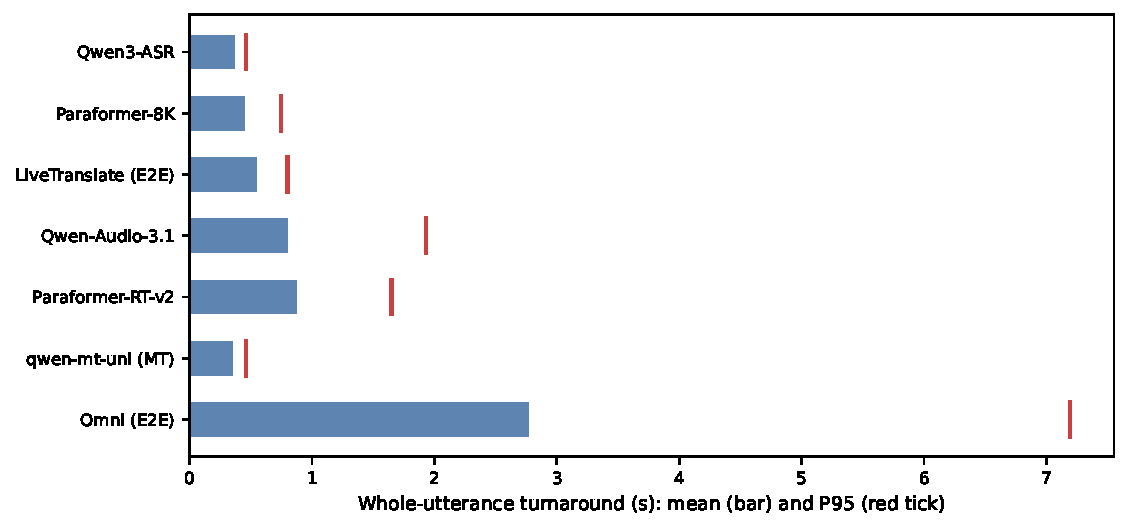
\includegraphics[width=0.5\textwidth]{../figures/fig7_latency.pdf}
\caption{API round-trip latency by system, mean and 95th percentile.}
\label{fig:latency}
\end{figure}

\section{Discussion}
\label{sec:discussion}

\subsection{Guidance for system integrators}

The measurements translate directly into selection guidance for practitioners
who compose commercial speech services. Above a signal-to-noise ratio of
about 5~dB, all five recognition systems deliver sub-percent to low-percent
error rates on clearly articulated speech, and the choice among them can be
driven by latency, cost, and interface ergonomics rather than accuracy. The
latency data in Table~\ref{tab:latency} then favour the LLM-ASR text-input
systems and the specialised streaming recognisers, which all answer in well
under a second, over the omni-modal path. Between 0 and 5~dB, the
architectural families separate: the degradation gradients in
Table~\ref{tab:slopes} show that every dB of noise costs a specialised streaming recogniser roughly four to five times what it costs an LLM-ASR system in Mandarin and about twice as much in English, so in
intermittently noisy environments such as public spaces, vehicles, or shared
offices, the foundation-model recognisers dominate the accuracy-latency
trade-off. Below 0~dB, no system transcribes English reliably, and the
appropriate response is architectural: capture improvement, multi-microphone
processing, or explicit rejection logic. For telephone-band audio, the
surprising result is that no specialist premium exists; the generalist
systems are as accurate in-band, and the telephone specialist is markedly
worse under reverberation, so its selection can be justified only by its
8~kHz interface requirements and its speed, not by accuracy.

For translation pipelines, the frontend hypothesis dominates all other
choices, and the latency data combine with it into a compact decision rule.
A cascade assembled from the fastest recognition tier and the text
translation engine completes in about 1.1 seconds per sentence at the mean,
roughly twice as fast as the omni end-to-end path, while the streaming
translation service completes in about half a second and is therefore the
natural choice when latency dominates; when noise robustness dominates, the
same streaming service and the LLM-frontend cascade lead the field, so the
two objectives point to the same shortlist. Swapping the recognition stage of a cascade from the specialised
streaming system to the LLM recogniser is worth 28 BLEU points at 0~dB on an
identical translation backend, which exceeds any reasonable expected gain
from changing the translation engine itself. The linear pass-through rule
quantified in Section~\ref{sec:results:cac}, at roughly half a BLEU point
per percentage point of recognition error, allows an integrator to rank
candidate frontends with recognition-only measurements, which are cheaper to
run and easier to interpret than full-pipeline evaluations, and to forecast
translation quality degradation from a measured or contracted recognition
error rate. The end-to-end versus cascade decision should rest on measured
degradation behaviour rather than architectural intuition: the omni-modal
end-to-end path evaluated here is simultaneously the slowest and, under
severe noise, the most fragile of the four translation designs, while a
dedicated streaming translation service achieves both the smallest relative
loss at 0~dB and sub-second latency.

\subsection{Why foundation-model recognisers degrade more slowly}

The robustness advantage of the LLM-ASR systems echoes the finding of
Radford et al.~\cite{radford2023robust} that recognition models trained on
very large and weakly curated corpora acquire substantial noise tolerance
without explicit multi-condition training. Two of our observations sharpen
this picture for API consumers. First, the advantage is strongly
condition-dependent: it is large under energetic babble noise and negligible
under codec, packet-loss, clipping, and tempo distortions, which barely
affect any system. This pattern is consistent with robustness arising from
exposure to diverse recording conditions during pre-training rather than
from any explicit enhancement front-end. Second, the advantage is
language-asymmetric, with Chinese recognition nearly immune at 0~dB while English recognition of the same systems fails at 37 to 50 percent. Providers
disclose neither training mixture nor per-language capacity, so the asymmetry
can only be documented, not explained, at the black-box level; the
documentation itself is actionable, since it implies that multilingual
deployments should be derated per language rather than per provider. It also implies a concrete procurement test: a
single-language noise probe, one hundred sentences of the target language
at 0~dB babble, is enough to place a candidate service on the robustness
spectrum documented here, and repeating the probe per deployment language
guards against extrapolating a strong Mandarin result to a weak English
result or the reverse. The direction decomposition of
Section~\ref{sec:results:cascade} extends the same caution to translation
deployments, where the two directions of a bilingual service degraded by
strikingly different amounts under identical noise.

\subsection{Cascade versus end-to-end revisited}

The classical comparison of Bentivogli et al.~\cite{bentivogli2018cascade}
found end-to-end and cascade systems competitive on clean speech with
different error structures. Our measurements extend that comparison to
degraded channels in the black-box setting and qualify it in two ways. The
end-to-end advantage in absolute quality against an independent reference is
real but partly a family artefact, since the omni system that translates
directly also shares a generation family with the strongest reference
producer, and the advantage inverts under the secondary reference, as
Section~\ref{sec:results:dual} shows. More importantly, robustness is not an
architectural property but a property of the acoustic frontend wherever it
lives. The end-to-end service with the specialised internal frontend is the
most resilient path we measured, while the end-to-end omni path is the most
fragile, and the same frontend ordering that explains cascade behaviour also
explains end-to-end behaviour. For a consumer, the practical question is not
which architecture to prefer but where the provider placed its best acoustic
model, and the answer is discoverable only by measurement of the kind this
benchmark performs.

\subsection{Methodological implications for black-box evaluation}

Three methodological observations generalise beyond the specific services
tested. The dual-reference protocol of Section~\ref{sec:results:dual}
demonstrates that machine-generated evaluation references can reorder
systems in a way that tracks reference-generator affinity rather than
translation quality, and that degradation-relative conclusions are the
stable currency of black-box comparison. The synthesis-based corpus design
gives black-box studies an exact transcript by construction, which matters
because at sub-percent clean error rates, transcription uncertainty in
recorded corpora would be comparable to the effects being measured. Finally,
the refusal behaviour documented in Section~\ref{sec:results:main}, where
one system returns empty output on a small but systematic subset of severely
degraded utterances, argues that black-box benchmarks should report response
completeness alongside error rates, since a missing transcript and a wrong
transcript have different downstream failure modes.

\subsection{A worked example of the pass-through rule}

The pass-through rule is most useful when stated as an explicit calculation.
Suppose an integrator operates a cascade built on the LLM recogniser in an
environment that occasionally degrades to 10~dB, at which the recogniser
errs at 0.9 percent, and contracts a translation stage equivalent to the one
measured here. The rule predicts a translation loss of roughly 0.47 times
0.9, that is 0.4 BLEU points, which is below the clean-condition agreement
between the two reference systems and therefore negligible. If the same
deployment used the specialised streaming recogniser, whose 10~dB error
rate is 2.8 percent, the predicted loss is 1.9 BLEU points, still modest,
but the margin to the 0~dB regime, where the rule predicts 27 to 38 points
of loss for the two frontends respectively, is thin. The rule therefore
both quantifies the mild regime, where no architectural action is needed,
and identifies the severity threshold beyond which the frontend choice
becomes the dominant design decision. The same arithmetic applied to the
measured error rates of a candidate system at the actual operating
signal-to-noise distribution of a deployment yields an expected translation
quality distribution without running the translation stage at all.

\subsection{Implications for evaluation practice and future work}

Beyond the specific findings, the benchmark design carries lessons for
future evaluations of commercial speech intelligence. A benchmark intended
to track black-box services over time should log every raw response rather
than only aggregate scores, because behavioural changes such as the refusal
pattern documented here appear as distributional shifts before they appear
in means. It should treat reference construction as a first-class
experimental variable, since Section~\ref{sec:results:dual} shows that the
reference generator can reorder systems. It should separate degradation
gradients, which generalise across severity, from point estimates, which do
not, and it should report response completeness alongside accuracy. The
present study points to four directions for follow-up work: replication
across providers to separate family effects from provider effects, extension
to spontaneous and accented speech, sweep-based characterisation of the
currently fixed-severity conditions, and human-reference scoring of the
translation stage to anchor the machine-reference comparisons. As foundation
model services begin to expose streaming speech interfaces with embedded
recognition, the measurement approach demonstrated here, treating each
service as an opaque function from degraded audio to text and scoring the
complete pipeline end to end, appears to be the only viable methodology for
the comparative robustness questions that practitioners actually face.

\section{Limitations}
\label{sec:limitations}

The benchmark uses synthetic speech from four neural voices. Synthetic
speech lacks the disfluencies, accents, emotional variation, and channel
noise of spontaneous human recordings, and although the exact-transcript
property is decisive for measurement at sub-percent error floors, clean
error rates measured on synthetic speech should not be read as population
estimates for human speech; the degradation deltas, which are the object of
this study, are less sensitive to this concern because they are within-system
contrasts. All systems come from a single provider, so architectural family
effects and provider effects are confounded; the family-level regularities
reported here are consistent with published training-scale
explanations~\cite{radford2023robust}, but cross-provider replication is
required before they can be attributed to architecture rather than to one
provider's engineering. The babble noise is itself synthesised from
disjoint neural voices, which makes it speech-shaped and fully reproducible
but smoother than real multi-talker cocktail-party interference, which
includes semantic competition and stronger nonstationarity. Severity levels
for the non-noise degradations were fixed at deployed-but-aggressive values
rather than swept, so only the noise family is characterised by a gradient.
Translation quality is measured with BLEU and chrF against machine-generated
references, with the family-affinity bias that
Section~\ref{sec:results:dual} quantifies; human-reference scoring would
strengthen absolute claims. Finally, commercial APIs are moving targets: the
measurements document the October 2026 versions of the listed services, and
one of the systems could not complete its full condition grid before its
free-tier quota was exhausted, which is itself a practically relevant datum
for anyone planning a similar measurement on complimentary quotas.

\section{Conclusions}
\label{sec:conclusions}

This paper introduced CascadeBench, a black-box benchmark that measures how
acoustic channel degradations propagate through commercial speech
recognition and translation services, and reported a complete measurement
over a controlled bilingual corpus of 480 sentences, fourteen degradation
conditions from seven families, and an eight-level noise severity sweep
from 20 to $-10$~dB, covering five recognition
systems from three product classes, three cascade translation paths,
and two end-to-end speech translation paths, all accessed through their
public interfaces on free service quotas; the central design was validated
on 150 human-recorded utterances under measured impulse responses and a
six-level real-babble ladder, a measured-RIR bridge condition on the
synthetic corpus, an open-weights locally executed recogniser, and a
second-vendor translation engine used as both a family-disjoint reference
and an alternative cascade backend.

The measurements support five conclusions. First, the product classes of
commercial recognisers differ in where they fail under noise, not merely how
fast: LLM-based recognisers hold a sub-percent floor and cross ten percent
error 2.2 to 2.5~dB later in Mandarin and 4.4 to 4.8~dB later in English
than the specialised streaming system, then collapse more sharply, and below
0~dB they fail by insertion-heavy hallucination with character error rates
above 100 percent; the real-speech validation reproduces this
knee-and-collapse structure and the hallucination regime, with three
calibrations: real rooms at matched reverberation time prove far milder
than the synthetic low-DRR stress response (and a measured telephone-band
specialist loses 3.4 rather than 18.2 percent under them), the LLM
noise-tolerance advantage holds only in the near-knee, low-error regime --
disappearing and for one LLM system reversing once error passes the
ten-percent level -- and is larger against real babble than synthetic
babble, and the Mandarin-insertion, English-deletion failure structure
replicates on an open-weights model outside the vendor, while
language-specific tolerance levels do not. Second, robustness is
condition- and language-specific
rather than uniform: narrowbanding, coding, packet loss, clipping, and tempo
changes at deployed severities are individually negligible for all systems,
0~dB babble nearly destroys English recognition for every system while
leaving the best Mandarin recognition low, and no system, of any class,
transcribes reliably below 0~dB. Third, the quality of a speech translation
cascade under degradation is governed by its recognition frontend, and the
relationship is an empirical linear pass-through of 0.44 to 0.54
BLEU points per percentage point of recognition error, with intercepts
statistically indistinguishable from zero, stable under leave-one-condition-out
refits for two of the three cascades, and honest condition-level
uncertainty that is substantially wider than the sentence-level intervals,
across up to fifteen conditions and three frontends; on real speech the
same relation holds with slopes of 0.43 (Mandarin) and 0.72 (English) over
nine conditions, and it survives swapping the translation engine for a
second vendor's model, which moves absolute scores by tens of BLEU points
but leaves the relative-loss trajectory nearly unchanged. Fourth,
end-to-end speech translation does not inherit
robustness automatically: the most resilient translation path measured is a
dedicated streaming end-to-end service, while the omni-modal end-to-end
path is the slowest and the most fragile of the end-to-end paths, degrading
more than the LLM-frontend cascades at 0~dB in point estimate under every
reference, with a margin that shrinks to under one point against the
Qwen3-ASR cascade under the oracle reference and whose paired interval
crosses zero there; on real speech the streaming end-to-end path likewise
loses a larger fraction of its clean quality under 0~dB real babble than a
well-frontended cascade, while the absolute BLEU ordering of the two paths
remains reference-dependent. Fifth,
black-box evaluation carries specific methodological obligations that this
benchmark operationalises, including three-reference scoring with one
family-disjoint reference to control machine-reference affinity -- under
which the relative-loss ranking is stable except for a sub-point inversion
between the omni path and the Qwen3-ASR cascade under the same-engine
reference -- exact-transcript corpora to enable sub-percent
measurement, the reporting of response completeness alongside error rates,
and the anchoring of service-level findings in measured signal properties,
which here exposed a sharp dissociation between intelligibility metrics and
recognition error across degradation families.

The benchmark recipe, including the corpus, the seeded degradation pipeline,
the degraded audio tree, all model responses, and the analysis code, is
released so that the measurement can be re-executed and verified as
providers update their services. The released artefacts are versioned alongside the service
identifiers and access dates of every system, so that future re-runs can
attribute score movements either to provider-side model updates or to
changes in the benchmark itself, a distinction that periodic evaluation of
moving targets requires. Together with the zero-cost execution protocol
described in Section~\ref{sec:methods}, the release is intended to make
robustness re-measurement a routine maintenance activity for speech
deployments rather than a one-off research exercise. As
speech intelligence continues to migrate into provider-operated black-box
systems, controlled measurement of this kind, repeated over time and across
providers, offers the community a practical substitute for the training-set
access that classical robustness research assumed, and offers integrators
the quantitative basis that architectural intuition alone cannot supply.

\appendix
\section{Corpus composition}
\label{app:corpus}

Table~\ref{tab:corpus} summarises the corpus structure and lists one sample
sentence per stratum. The four domains are constructed to differ in register,
vocabulary, and numerical density. The broadcast-news domain uses formal
written register with institutional vocabulary, the conversation domain uses
colloquial everyday phrasing, the technical domain uses scientific and
engineering terminology, and the numerals-and-entities domain concentrates
dates, times, quantities, prices, addresses, codes, and named entities, with
all numbers written out in words as described in
Section~\ref{sec:methods}. Length strata are defined per language as short,
medium, and long as given in Section~\ref{sec:methods}, and every
domain-by-length cell contains twenty sentences per language, giving 240
sentences per language and 480 in total. The severity sweep subset of 144
sentences is sampled evenly across all cells, six sentences per cell per
language.

\begin{table}[h]
\centering
\caption{Corpus structure with one sample sentence per domain.}
\label{tab:corpus}
\small
\begin{tabular}{lp{8.8cm}}
\toprule
Domain & Sample sentence \\
\midrule
News (zh) & 国家统计局今天发布了上月经济运行数据。 \\
News (en) & The central bank raised interest rates by twenty five basis points to curb inflation. \\
Conversation (zh) & 我打算下班之后去健身房锻炼一个小时。 \\
Conversation (en) & I was thinking we could drive to the beach this weekend if the weather holds. \\
Technical (zh) & 混响是声波在房间内多次反射形成的，会显著降低远场语音识别的准确率。 \\
Technical (en) & Reverberation arises when sound waves reflect repeatedly off room surfaces. \\
Numerals (zh) & 从北京到上海的高铁大约需要四个半小时。 \\
Numerals (en) & The high speed train from Beijing to Shanghai takes about four and a half hours. \\
\bottomrule
\end{tabular}
\end{table}

\section{Qualitative error analysis}
\label{app:qualitative}

Table~\ref{tab:examples} collects representative model responses that
illustrate the failure patterns behind the aggregate numbers in
Section~\ref{sec:results}.

The refusal behaviour of Section~\ref{sec:results:main} is shown in the
first row: under 0~dB babble the Qwen-Audio recogniser returns an empty
transcript for a substantial English sentence, which the benchmark scores as
a complete failure. The second row shows the opposite regime: the same
system, on a long English news sentence at the same severity, produces a
verbatim transcript, which underlines how bimodal the sentence-level
distributions of Fig.~\ref{fig:dist} are. Row three shows the dominant error
mode of the specialised streaming recogniser under severe noise, where most
of the sentence is lost and only a short fragment survives. Row four shows a
typical near-miss of the LLM recogniser in Chinese, where a single
content word, density, is replaced by another word of similar phonetic
shape, speed, without any structural damage. Row five shows the collapse of
the telephone-band specialist under reverberation, which occasionally
produces short disconnected fragments rather than transcripts. Row six
shows an error that the recognition stage never sees but the translation
consumer experiences: under 0~dB noise the omni end-to-end path substitutes
a plausible but wrong entity, rendering the sports centre of the source as a
grand theatre, a hallucination that a string-matching metric penalises only
lightly but that is catastrophic for factual fidelity. Row seven shows the
narrowband immunity of the LLM recogniser, which returns a verbatim
transcript of telephone-band audio. Together the examples support the
reading of Section~\ref{sec:discussion}: the systems differ less in whether
they fail than in how, and the failure modes, from verbatim robustness to
silent entity substitution to outright refusal, have distinct downstream
consequences.

\begin{table}[h]
\centering
\caption{Representative system responses under degradation.}
\label{tab:examples}
\small
\begin{tabular}{llp{6.1cm}}
\toprule
Condition & System & Reference and response \\
\midrule
0 dB, en & Qwen-Audio-3.1 & Reference: Police arrested two suspects on Tuesday. Response: empty transcript. \\
0 dB, en & Qwen-Audio-3.1 & Reference: The transport minister told reporters on Friday that the government would invest heavily in electric vehicle charging infrastructure. Response: verbatim transcript. \\
0 dB, en & Paraformer-RT-v2 & Reference: The battery lasts twenty hours. Response: About. \\
0 dB, zh & Qwen-Audio-3.1 & Reference: 这款处理器的晶体管密度提升了近一倍。 Response: 这款处理器的晶体管速度提升了近一倍。 \\
Reverb, zh & Paraformer-RT-8K & Reference: 记者从发布会上了解到，本次合作项目将覆盖全国二十多个主要城市。 Response: 七月同。非常了解到。 \\
0 dB, E2E & Omni-Flash & Source: 新建成的体育中心可容纳六万名观众。 Translation: The newly built Grand Theatre can accommodate 60,000 audience members. \\
Narrow, en & Qwen-Audio-3.1 & Reference: This coffee shop is cozy. Response: verbatim transcript. \\
$-10$ dB, en & Qwen-Audio-3.1 & Reference: The battery lasts twenty hours. Response: fluent unrelated Chinese text of several sentences (hallucination). \\
\bottomrule
\end{tabular}
\end{table}

\section{Cross-system text normalisation}
\label{app:normalisation}

Comparing transcripts across commercial recognisers requires a normalisation
protocol that neutralises provider-specific inverse text normalisation. The
protocol applies the following rules identically to references and
hypotheses, in order. Unicode compatibility folding and case folding are
applied first, and punctuation is removed. Numeric expressions are then
canonicalised to digit form on both sides. For Chinese, the rules handle
cardinal numbers with the standard multipliers, digit-by-digit readings such
as room and code numbers where each digit is read separately, decimal
fractions written with the point particle, time-of-day expressions in which
the hour and minute parts are converted separately, percentage markers,
which are deleted on both sides, and scale multipliers, where a digit
followed by wan, yi, or their combinations is expanded to the full
multiplied-out form, so that twenty-six million written as 2600万 in one
system's output and as 26000000 in another's both canonicalise identically.
For English, the rules handle cardinal numbers including compound
hyphenated forms and the and connector, time and digit-by-digit readings
such as twelve zero eight and nine forty, which canonicalise to 1208 and
940, decimal fractions expressed with point, scale multipliers from thousand
to trillion, and ordinal expressions of both word and digit form, which are
masked to a common placeholder since their spoken-to-written realisations
differ across systems in ways that carry no acoustic information. The rule
set was developed and frozen by inspecting all high-error sentences of the
clean condition until no residual mismatches attributable to normalisation
remained, a procedure that could in principle favour whichever system's
conventions dominate the clean outputs, so a sensitivity analysis was run:
re-scoring the main grid with case and punctuation folding only, dropping
numeral canonicalisation entirely, raises clean-condition error rates from
0.5, 2.3, and 0.3 percent to 6.1, 6.2, and 0.8 percent for Qwen-Audio,
Paraformer, and Qwen3-ASR respectively, while the 0~dB scores move by less
than 1.5 points and the system ordering is unchanged in every condition.
The normalisation therefore compresses but does not create the reported
system differences, and the residual protocol noise on clean speech is
bounded above by the strongest system's per-language clean rate of 0.14
percent in Mandarin (0.29 percent pooled over both languages), with the
caveat that the two systems most affected by numeral conventions differ
most under the raw protocol. The full normalisation code is released with
the benchmark.



\section*{Data and code availability}
The complete benchmark is publicly released at
\url{https://github.com/43aquarius/CascadeBench-Paper-AppliedAcoustics}:
the sentence corpus, the seeded perturbation implementations, the full
degraded audio tree, all per-sentence model transcripts and translations
(33{,}000 logged API responses), the analysis scripts, and the LaTeX source
of this manuscript. Every number and figure in the paper is regenerated
from the released logs by the released analysis scripts. An anonymised
snapshot for reviewers is provided with the submission.

\section*{Declaration of generative AI and AI-assisted technologies in the
writing process}
During the preparation of this work the authors used a large language model
assistant in the development of the analysis scripts and in drafting
revisions of the manuscript text, in order to accelerate the benchmark
construction and to improve the readability of the presentation. The
experimental measurements, the analysis decisions, and the verification of
all reported numbers against the released logs were performed and checked by
the authors, who take full responsibility for the content of the published
article.

\section*{Declaration of competing interest}
The authors declare that they have no known competing financial interests or
personal relationships that could have appeared to influence the work reported
in this paper.

\bibliographystyle{elsarticle-num}
\bibliography{refs}

\end{document}
